% !TeX encoding = UTF-8
% !TeX program = pdfLaTeX
% !TeX root = matlab-exercises-emaip.tex
% !TeX spellcheck = en_GB
\section{Functions and recap}
\SetExerciseDirectory{09_functions}

\subsection{Plotting and normalizing data}

\begin{ex} \label{exComparingRawDataSets}%
Four datasets with amplitude over time have been 
placed in your git repository in the location
\verb!18_dealing_with_experimental_data/data!.
Plot these four datasets in one figure.
\begin{hint}
Load the datasets one by one at the time using the \verb!dlmread! function.
For each dataset extract the x and y values (first and second column).
Plot the x and y values.
\end{hint}
\begin{sol}
A solution is:
\begin{lstlisting}
data = dlmread('data/dataset_01.csv');
x = data(:, 1);
y = data(:, 2);

figure(1);
clf;
plot(x, y);
hold on;

data = dlmread('data/dataset_02.csv');
x = data(:, 1);
y = data(:, 2);
plot(x, y);

data = dlmread('data/dataset_03.csv');
x = data(:, 1);
y = data(:, 2);
plot(x, y);

data = dlmread('data/dataset_04.csv');
x = data(:, 1);
y = data(:, 2);
plot(x, y);
\end{lstlisting}
\end{sol}
\end{ex}


\begin{ex}
Improve the plotting of the datasets in exercise 
\ref{exComparingRawDataSets} by normalizing the data
in the following way.
In this exercise you will probably have to repeat the plots 
multiple times and locate specific values in the plot using the
\emph{Data Tips} tool in the plot window.

Shift the x values such that the initial value (at $x = 0$) is
at a maximum.
Scale the y values such that the initial value (at $x = 0$) is one.
Then scale the x values such that one full oscillation of the
system has occurred at $x = 1$.
After shifting and scaling the plotted data should 
have local maxima at $x = 0$, $x = 1$, $x = 2$, $x = 3$, \ldots

The purpose of the normalizations is to make it easier to 
compare datasets acquired under different conditions.
\begin{hint}
To shift the x values a fixed value should be subtracted from the x 
value.
To scale the y values it should be divided with a fixed value.
To scale the x values it should be divided with a fixed value.
\end{hint}
\begin{sol}
A solution is:
\begin{lstlisting}
%%
data = dlmread('data/dataset_01.csv');
x = data(:, 1);
y = data(:, 2);
figure(5)
clf;
first_peak = -1.255;
cycle_length = 1.526;
peak_value = 0.87;
plot((x-first_peak) / cycle_length, y / peak_value);
hold on;
%xlim([0, 6]);

%%
data = dlmread('data/dataset_02.csv');
x = data(:, 1);
y = data(:, 2);
figure(5)
first_peak = -1.447;
cycle_length = 2.859 / 2;
peak_value = 1.05;
plot((x-first_peak) / cycle_length, y / peak_value);

%%
data = dlmread('data/dataset_03.csv');
x = data(:, 1);
y = data(:, 2);
figure(5)
first_peak = -0.9429;
cycle_length = 4.552 / 4;
peak_value = 1.25;
plot((x-first_peak) / cycle_length, y / peak_value);

%%
data = dlmread('data/dataset_04.csv');
x = data(:, 1);
y = data(:, 2);
figure(5)
first_peak = -1.892;
cycle_length = 3.243 / 5;
peak_value = 2.3;
plot((x-first_peak) / cycle_length, y / peak_value);
\end{lstlisting}
\end{sol}
\end{ex}



\begin{ex}
\begin{tcolorbox}
This exercise is meant as a challenge, it is much more difficult 
than the standard exercises.
Consider this an optional exercise, you do not have to 
solve it.
\end{tcolorbox}
Locate the file \verb!18_dealing_with_experimental_data/mystery_function.m! and figure out what the function actually does 
(and how).
\begin{hint}
Try to plot information from inside the function.
You an also try to rename the variable names, so they 
become more meaningful.
\end{hint}
\begin{sol}
No solution provided.
\end{sol}
\end{ex}



\subsection{Function handles}

We have earlier worked with functions that take numbers and lists 
as input arguments.
But a function can also take a function handle as input argument.
A function handle is a reference to a specific function. 
In the example below is a reference to the sinus function created 
and later tested.
%
\begin{lstlisting}
>> functionHandle = @sin;
>> functionHandle(0.123)
ans = 0.1227
>> sin(0.123)
ans = 0.1227
\end{lstlisting}
%
A function handle can also be generated without using an existing function as template.
The following syntax lets you create function handles from scratch.
%
\begin{lstlisting}
@(input parameters) code to calculate result
\end{lstlisting}
%
As an example the second order Taylor expansion for $\cos(x)$ 
is used to create a function handle.
\begin{lstlisting}
>> fh = @(x) 1 - 0.5*x.^2;
>> cos([0, 0.1, 0.3])
ans = 1.0000    0.9950    0.9553
>> fh([0, 0.1, 0.3])
ans = 1.0000    0.9950    0.9550
\end{lstlisting}

\begin{ex}
Create a function handle named \emph{sumOfSineAndCosine} for the expression
\begin{align*}
f(x) & = \sin(x) + \cos(x)
\end{align*}
Example usage of the function:
\begin{lstlisting}
>> sumOfSineAndCosine([0, 0.1, 0.2, 0.3, 1])
ans = 1.0000    1.0948    1.1787    1.2509    1.3818
\end{lstlisting}
\begin{hint}
Use the syntax
\begin{lstlisting}
fname = @(x) expression;
\end{lstlisting}
Where \verb!fname! and \verb!expression! should be modified.
\end{hint}
\begin{sol}
To create the function handle, run the code below in the matlab command window.
\begin{lstlisting}
sumOfSineAndCosine = @(x) sin(x) + cos(x);
\end{lstlisting}
\end{sol}
\end{ex}



\begin{ex}
Create a function that takes a function handle and a list as input arguments.
The output should be a list with the same number of elements as the input list.
The values in the output list should be the value returned by the function handle 
when applied to the corresponding element in the input list.
The function signature should be:
\begin{lstlisting}
function res = applyFunctionHandleToList(fh, list)
\end{lstlisting}
Example usage of the function:
\begin{lstlisting}
>> applyFunctionHandleToList(@(x) 1, [1, 3, 9])
ans = 1     1     1
>> applyFunctionHandleToList(@(x) 1-x, [1, 3, 9])
ans = 0    -2    -8
\end{lstlisting}
\begin{hint}
Use a for loop to iterate over the input list.
\end{hint}
\begin{sol}
A solution is:
\begin{lstlisting}
function res = applyFunctionHandleToList(fh, list)

res = list;
for idx = 1:length(list)
	res(idx) = fh(list(idx));
end

end
\end{lstlisting}
\end{sol}
\end{ex}


\subsection{Things from old exam sets}

\begin{ex}
Create a function that calculates the n'th Fibonacci number. The nth
fibonacci number can be calculated using the formula: 
\[
F_n = F_{n-1} + F_{n-2}
\]
with the two base cases $F_0 = 0$ and $F_1 = 1$. The sequence goes like
$0, 1, 1, 2, 3, 5, 8, 13, 21, 34, ...$
\begin{lstlisting}
function res = fib(n)
\end{lstlisting}
Example usage of the function:
\begin{lstlisting}
>> fib(0);
>> fib(0)
ans = 0
>> fib(1)
ans = 1
>> fib(6)
ans = 8
>> fib(17)
ans = 1597
>> fib(29)
ans = 514229
\end{lstlisting}
\begin{hint}
Use one or more if statements to ensure that the two base
cases are handled properly.
Then use the relation
\[
\textrm{fib}(n) = \textrm{fib}(n - 1) + \textrm{fib}(n - 2)
\]
\end{hint}
\begin{sol}
A solution is:
\begin{lstlisting}
function res = fib(n)

if(n < 2)
  res = n;
else
  res = fib(n - 1) + fib(n - 2);
end
end
\end{lstlisting}
\end{sol}
\begin{solutionfile}{fib_test.m}
function tests = fib_test
    tests = functiontests(localfunctions);
end


%% The Fibonacci sequence
% Create a function that calculates the n'th Fibonacci number. The nth
% fibonacci number can be calculated using the formula: 
% F_n = F_{n-1} + F_{n-2}
% with the two base cases F_0 = 0 and F_1 = 1. 
% The sequence goes like 0, 1, 1, 2, 3, 5, 8, 13, 21, 34, ...
% The function should have the signature
% function res = fib(n)

%% Test 1: Identical inputs
function test1(testCase)
    actual_value = fib(0);
    expected_value = 0;
    testCase.verifyEqual(actual_value, expected_value);
end
function test2(testCase)
    actual_value = fib(1);
    expected_value = 1;
    testCase.verifyEqual(actual_value, expected_value);
end
function test3(testCase)
    actual_value = fib(2);
    expected_value = 1;
    testCase.verifyEqual(actual_value, expected_value);
end
function test4(testCase)
    actual_value = fib(6);
    expected_value = 8;
    testCase.verifyEqual(actual_value, expected_value);
end
function test5(testCase)
    actual_value = fib(17);
    expected_value = 1597;
    testCase.verifyEqual(actual_value, expected_value);
end
function test6(testCase)
    actual_value = fib(29);
    expected_value = 514229;
    testCase.verifyEqual(actual_value, expected_value);
end
\end{solutionfile}
\begin{solutionfile}{fib.m}
function res = fib(n)

if(n < 2)
  res = n;
else
  res = fib(n - 1) + fib(n - 2);
end
end
\end{solutionfile}
\end{ex}





% 2020-01-24 Reexam
\begin{ex}
Recreate the figure below:
\begin{center}
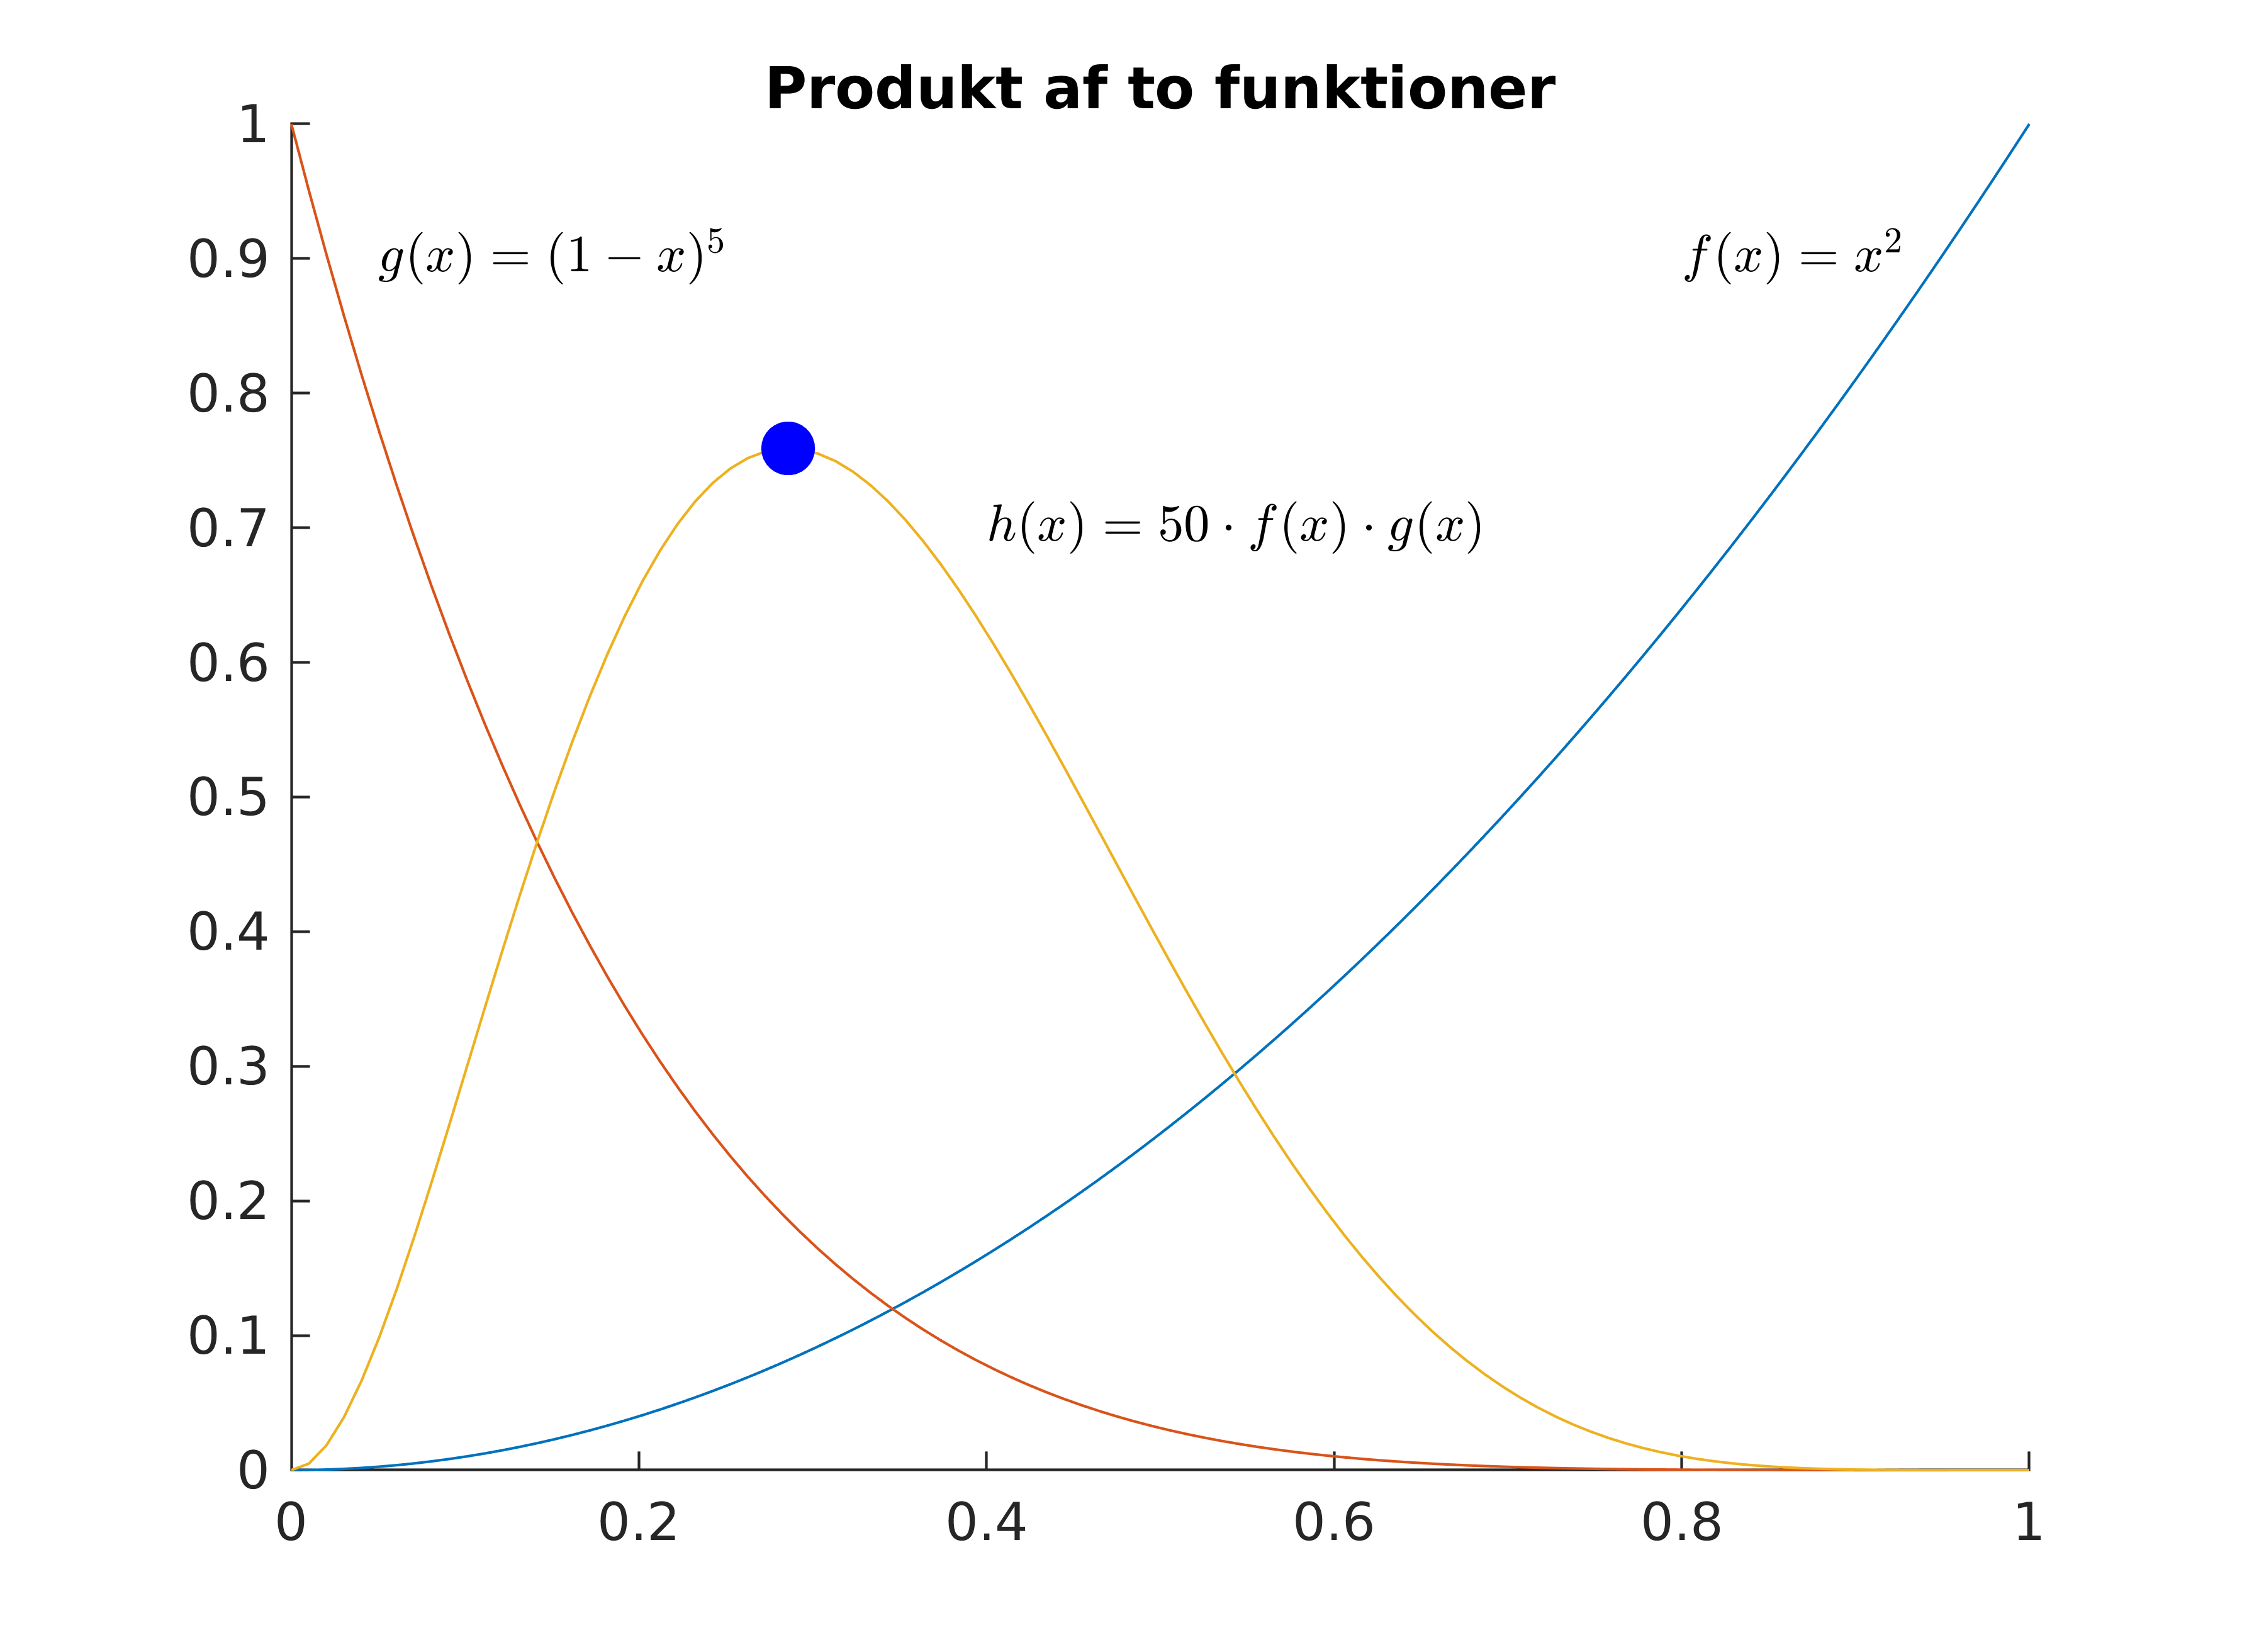
\includegraphics[width=0.7\textwidth]{pic/product_of_two_functions.png}
\end{center}
\begin{hint}
\end{hint}
\begin{sol}
A solution is:
\begin{lstlisting}
% Exercise 1: Recreate a figure

% Define f(x), g(x) and the range of x values that should be plotted.
fh = @(x) x.^2;
gh = @(x) (1-x).^5;
hh = @(x) 50*fh(x) .* gh(x);
xvals = linspace(0, 1);

% Locate minima of h(x).
h_minima = fminsearch(@(x) -hh(x), 0.2);

% Start a new figure
figure(1);
clf;
hold on;

% Plot functions.
plot(xvals, fh(xvals));
plot(xvals, gh(xvals));
plot(xvals, hh(xvals));

% Indicate locations of roots.
plot(h_minima, hh(h_minima), '.b', 'MarkerSize', 35);

% Add text to plot.
text(0.8, 0.9, "$f(x) = x^2$", ...
    'interpreter', 'latex');
text(0.05, 0.9, "$g(x) = (1-x)^5$", ...
    'interpreter', 'latex');
text(0.4, 0.7, "$h(x) = 50 \cdot f(x) \cdot g(x)$", ...
    'interpreter', 'latex');

% Add title and axis labels.
title("Produkt af to funktioner");
%xlabel('x akse');
%ylabel('y akse');
ylim([0, 1]);

% Write the figure to disk.
print('product_of_two_functions.png', '-dpng', '-r600');
\end{lstlisting}
\end{sol}
\end{ex}







\begin{ex}
Determine the value of the following definite integral:
\begin{align*}
\int_0^1 x^2 \cdot  (1 - x)^5 \; dx
\end{align*}
Then determine the value of $\alpha$, which solves the 
equation below.
\begin{align*}
\frac{1}{2} \cdot \int_0^1 x^2 \cdot  (1 - x)^5 \; dx = \int_0^\alpha x^2 \cdot  (1 - x)^5 \; dx
\end{align*}
\begin{hint}
\end{hint}
\begin{sol}
A solution is:
\begin{lstlisting}
format long

hh = @(x) x.^2 .* (1-x).^5;

val = integral(hh, 0, 1)
integral(hh, 0, 0.3205189672974762) / val

%%
temp = @(x) integral(hh, 0, x) - 0.5 * val;
fzero(temp, 0.5)

format short
\end{lstlisting}
\end{sol}
\end{ex}

\begin{ex}
Create a function that classifies triangles into a set of
types according to their side lengths.
The function should have the signature:
\begin{lstlisting}
function res = triangle_type(a, b, c)
\end{lstlisting}
The input to the function is the length of the 
three sides of the triangle in increasing order ($a \le b \le c$).
The triangle types that should be recognized are:
\begin{description}
\item[impossible] it is not possible to construct a triangle with the given side lengths: $a + b < c$.
\item[equilateral] all sides in the triangle has the same length
\item[obtuse] has an angle above 90 degrees, has the property $a^2 + b^2 < c^2$
\item[right] one of the angles is precisely 90 degrees and the side lengths has the property $a^2 + b^2 = c^2$
\item[acute] all angles are below under 90 grader, the triangle has the property $a^2 + b^2 > c^2$
\end{description}
Use the following examples to test the function
\begin{lstlisting}
>> triangle_type(1, 2, 4)
ans = 'impossible'
>> triangle_type(2, 3, 4)
ans = 'obtuse'
>> triangle_type(3, 4, 5)
ans = 'right'
>> triangle_type(3, 3, 3)
ans = 'equilateral'
>> triangle_type(3, 3, 4);
>> triangle_type(3, 3, 4)
ans = 'acute'\end{lstlisting}
\begin{hint}
\end{hint}
\begin{sol}
A solution is:
\begin{lstlisting}
\end{lstlisting}
\begin{solutionfile}{triangle_type.m}
function res = triangle_type(a, b, c)
% Assume a < b < c

if(c - a - b > 0)
    res = 'impossible';
else
    if(abs(a - c) < 0.0000001)
        res = 'equilateral';
    else
        value = a^2 + b^2 - c^2;
        if(value > 0)
            res = 'acute';
        else
            if(value < 0)
                res = 'obtuse';
            else
                res = 'right';
            end
        end
    end
end
end
\end{solutionfile}
\end{sol}
\end{ex}


\pagebreak[4]
\subsection{Multiple plots in one}

It is possible to put multiple plots 
next to each other in a single plot in matlab.
This can be done using the subplot command.
The plot shown below
was generated by the code next to it.
\begin{multicols}{2}
\begin{lstlisting}
x = linspace(-5, 5);

figure(1);
clf;

subplot(2, 1, 1);
plot(x, sin(x));
title('Sin(x)');
ylim([-1.5, 1.5]);

subplot(2, 1, 2);
plot(x, x);
hold on;
plot(x, sin(x));
title('Taylor 1');
ylim([-1.5, 1.5]);
\end{lstlisting}
\columnbreak
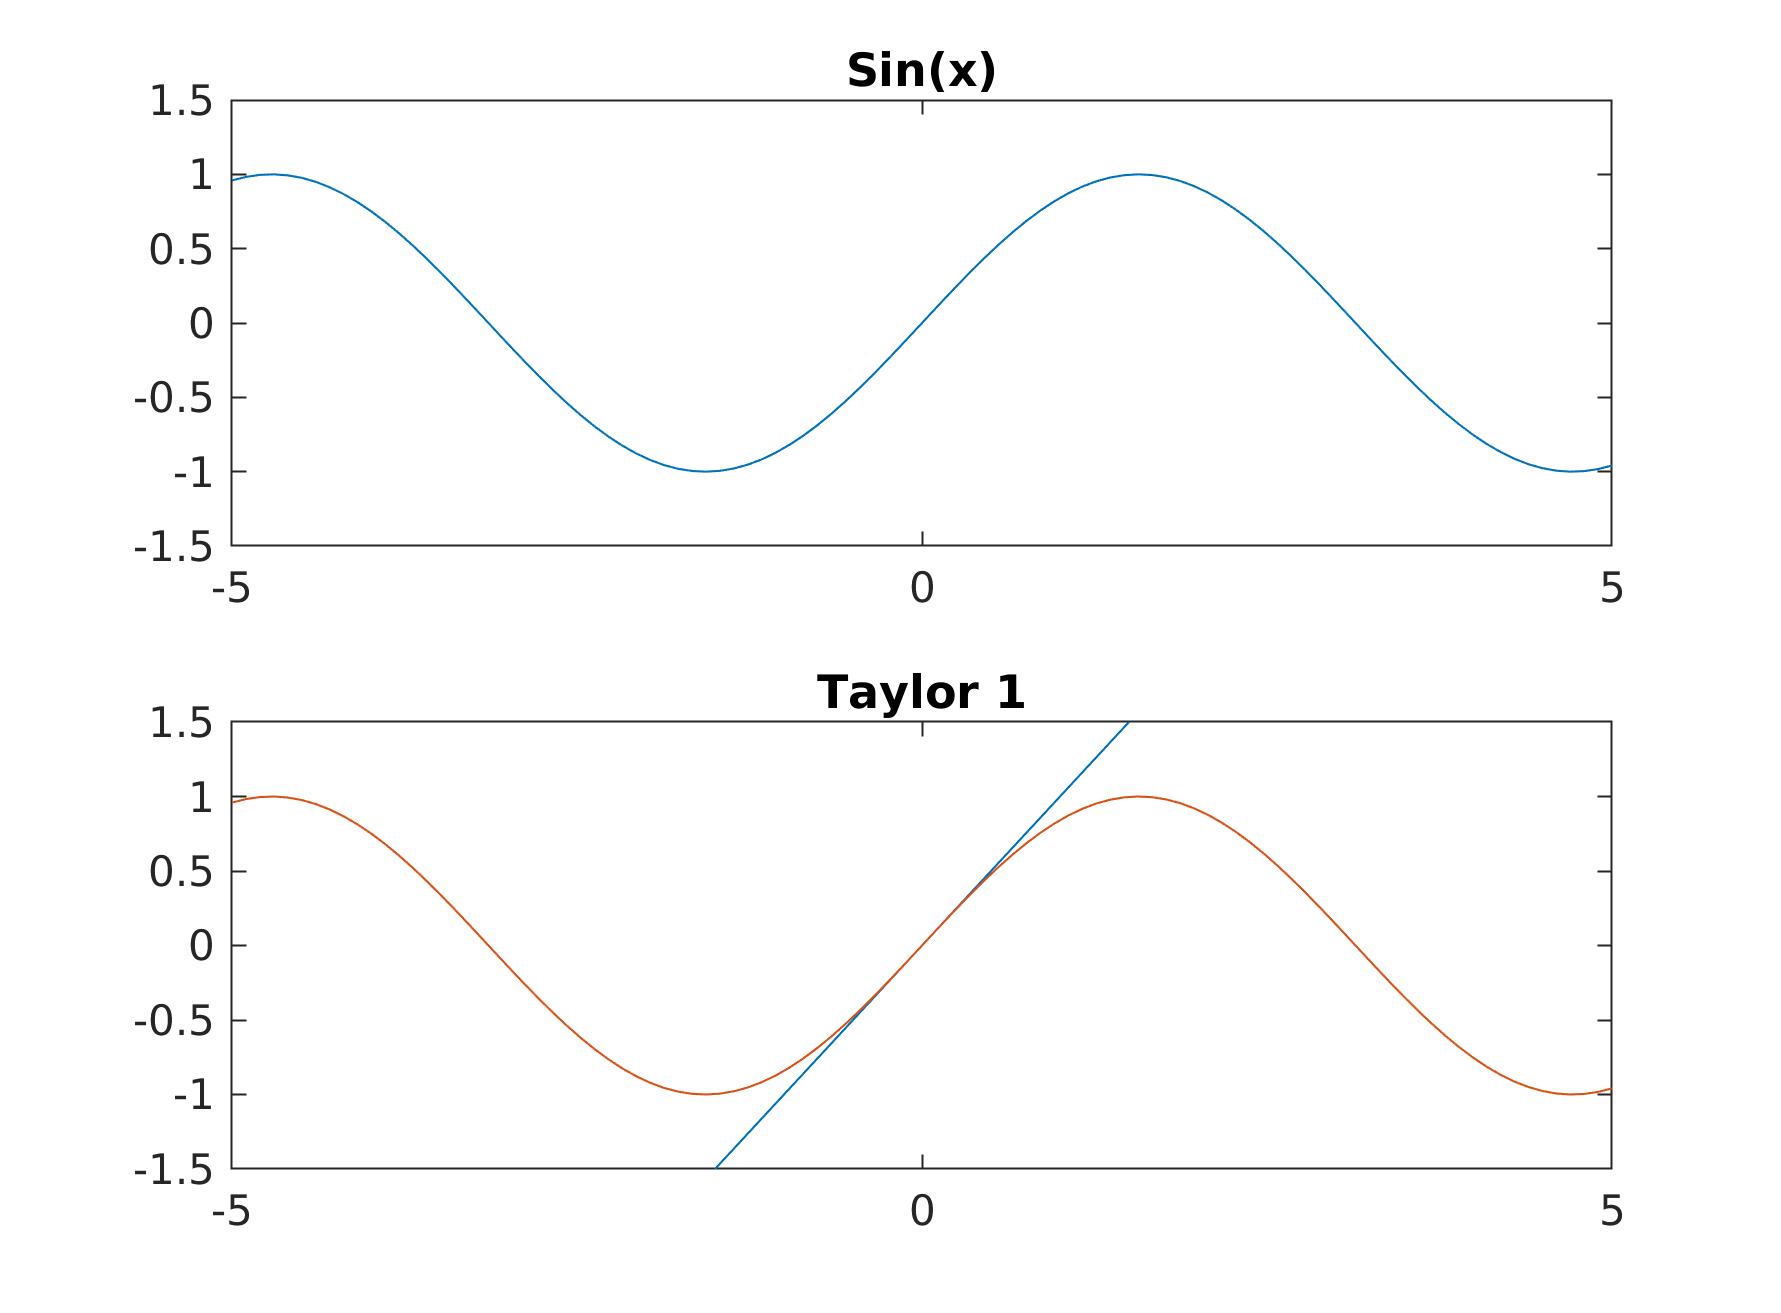
\includegraphics[width=\linewidth]{pic/subplot_example_1.png}
\end{multicols}

The three input parameters to the \verb!subplot! command
are as follows: 
\begin{itemize}
\item		the number of rows of subplots in the plot
\item		the number of columns of subplots in the plot
\item		a number indicating the subplot in which the following plot commands will operate.
\end{itemize}
The subplots are numbered row wise, so in a subplot 
with two rows and three columns, the subplot numbers will be
distributed as follows:
\begin{align*}
\begin{matrix}
1 & 2 & 3 \\
4 & 5 & 6
\end{matrix}
\end{align*}




\begin{ex}
Recreate the following plot: 
\begin{center}
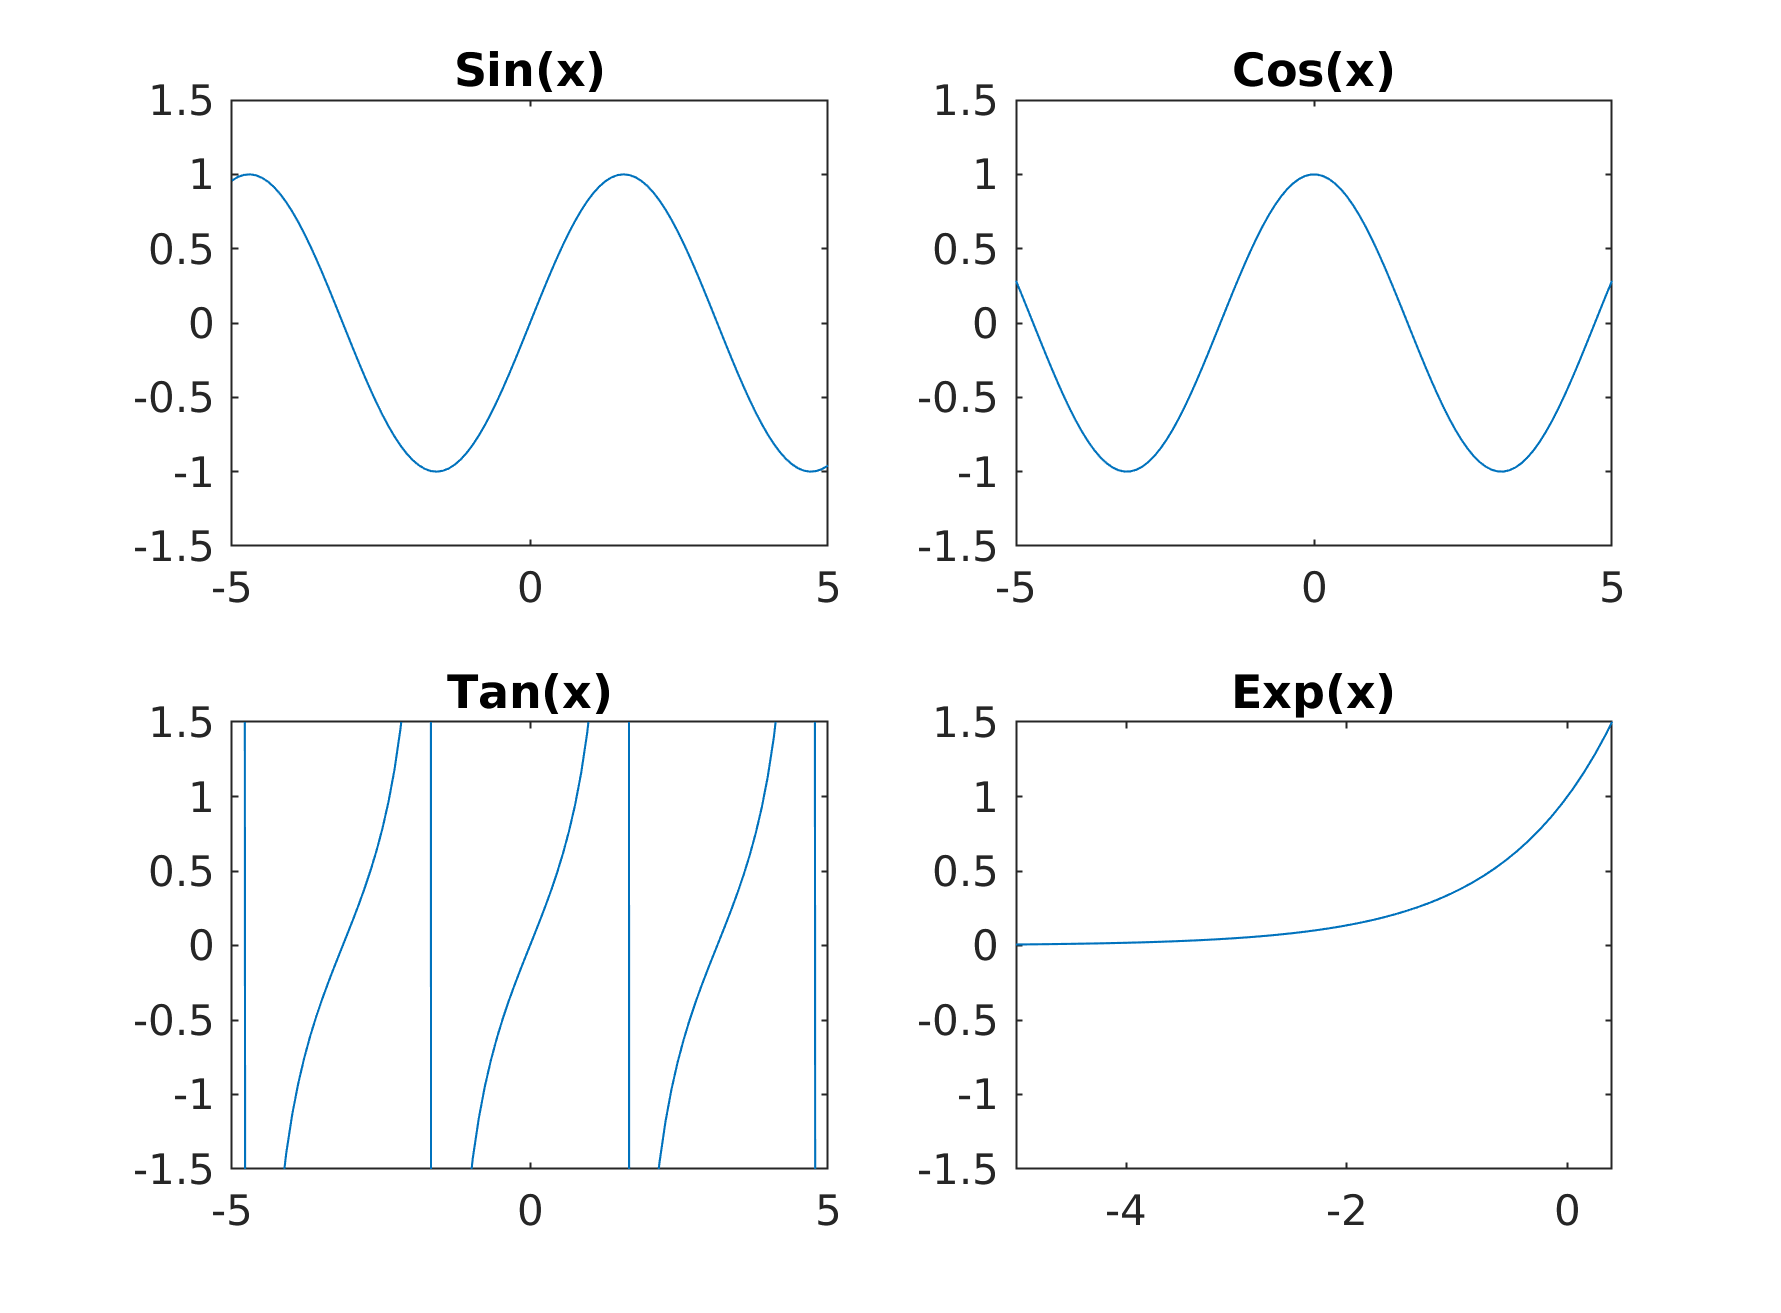
\includegraphics[width=9cm]{pic/subplot_exercise_1.png}
\end{center}
\begin{hint}
\end{hint}
\begin{sol}
A solution is:
\begin{lstlisting}
\end{lstlisting}
\end{sol}
\end{ex}
 